\chapter*{Questão 2}

\section*{Enunciado}

\noindent 2. Vamos considerar agora o problema de andarilhos aleatórios em uma dimensão. 
Aqui, em cada unidade de tempo, cada caminhante, independentemente onde esteja, 
dá um passo à direita (esquerda) com probabilidade $p$ ($q = 1 - p$). 
O caso $p = q = 1/2$ corresponde a um caminhante tão desnorteado que ele não 
se lembra de onde veio e nem qual o rumo certo a tomar. 
O caso em que $p \neq q$ corresponde ao viajante aleatório em uma ladeira. 
A questão nesta tarefa é calcular $\langle x \rangle$ e $\langle x^2 \rangle$ 
após um certo número $N$ de passos.

\begin{enumerate}
    \item[(a)] Considere $p = q = \tfrac{1}{2}$ e um número grande $M$ de andarilhos 
    todos partindo da origem ($x = 0$) no tempo inicial ($t = 0$). 
    Após $N = 1000$ passos faça um histograma do número de andarilhos $n(x)$ em função de $x$. 
    Que tipo de curva você obteve? Calcule $\langle x \rangle$ e $\langle x^2 \rangle$.

    \item[(b)] Refaça o item anterior considerando $p = \tfrac{1}{3}, \tfrac{1}{4}, \tfrac{1}{5}$. 
    Qual seria a forma analítica em termos de $N$, $p$ e $q$ para 
    $\langle x \rangle$ e $\langle x^2 \rangle$?
\end{enumerate}

\section*{Métodologia}

\subsection*{Referencial teórico questão 2}

Nos próximos projetos é pedido para calcular a média de passos de um \textit{andarilho aleatório}, ou seja, uma pessoa que não segue um padrão nas suas passadas, nessa simulação o indivíduo tem apenas um grau de liberdade, ou seja, ele só pode andar para direita ou esquerda. Vale notar, que é fixado uma probabilidade do andarilho dar um passo para direita como sendo, \textit{p}, portanto, a probabilidade desse indivíduo dar um passo a esquerda é \( q = 1 -p\).

\begin{equation} \label{equation_2}
    p(n_d) = \frac{N!}{n_d! n_e!} p^{n_d} q^{n_e}
\end{equation}

Desse modo, se a probabilidade de dar um passo para a direita é dada pela Equação \ref{equation_2}, onde $N$ é o número total de passos, $n_d$ é o número de passos a direita e $n_e$ é o número de passos a esquerda, a conta para $p(n_e)$ segue a mesma fórmula.

Assim sendo, é possível encontrar a média do números de passos a direita como sendo o número de passos totais multiplicado pela probabilidade do andarilho dar um passos a direita.

\begin{equation}\label{equation_3}
    <n_d> = \sum_{n_d=0}^{N} n_d \cdot p(n_d)
\end{equation}

\noindent Utilizando as Equações \ref{equation_3} e \ref{equation_2}, temos que,

\[     <n_d> = \sum_{n_d=0}^{N} n_d \frac{N!}{n_d! n_e!} p^{n_d} q^{n_e}  \]

\noindent utilizando o teorema dos binômios podemos reescrever a equação da seguinte maneira,

\[ <n_d> = \sum_{n_d=0}^{N} \binom{N}{n_d} p^{n_d} q^{n_e}\]

\noindent o que é equivalente a,

\[ F(p,q) = (p + q)^N\]
\noindent portanto,

\[ <n_d> = p \frac{\partial F(p,q)}{\partial p}\ = p N (p+q)^N \]

\noindent se $p + q = 1$, então:

\[ <n_d> = pN\]

Por fim, para $n_e$, $<n_e> = qN$. Além disso, para realizar o cálculo da média de passos totais, é necessário subtrair $<n_e>$ e $<n_d>$, \(<x> = <n_d> - <n_e>\), tendo em vista que no referencial escolhido a esquerda é considerado como sentido negativo. Ademais, para encontrar a média quadrática de passos $<x^2>$ é necessário utilizar as mesmas equações, porém, utilizando a segunda derivada parcial da função $F(p,q)$, realizando essas derivações temos que, \( <x^2> = 4 N p q\). Assim sendo, encontramos as equações \ref{média} e \ref{média quadrática} que nos dão a média de passos do andarilho e a média quadrática respectivamente.

\begin{equation} \label{média quadrática}
    <x^2> = 4 N p q
\end{equation}

\begin{equation} \label{média}
    <x> = N(p - q)
\end{equation}

\section*{Código}

Função principal do código, nela eu dou o número de bêbados, o número de passos e a probabilidade de dar um passo a direita.

\vspace*{2\baselineskip}



\begin{figure}[h!]
\centering
\caption{Função principal do código.}
\centering
\begin{lstlisting}
program main

  ! Eu vou definir as constantes
  m = 1e4 ! Número de bebados
  n = 1e2 ! Número de passos
  p = 0.33 ! Probabilidade de andar para direita
  x = calc(n,m,p)

end program main
\end{lstlisting}

\caption*{Fonte: Compilado pelo Autor.}
\label{fig:função_principal do_código tarefa 2}
\end{figure}

A função \texttt{calc}, implementada em Fortran77, realiza uma simulação de 
caminhantes aleatórios em uma dimensão, também conhecida como \textit{random walk}. 
A ideia do programa é acompanhar o movimento de um grande número de caminhantes 
independentes, cada um partindo da origem e dando uma sequência de passos para 
a direita ou para a esquerda, de acordo com uma probabilidade pré-definida.

O funcionamento pode ser descrito da seguinte maneira: inicialmente, o vetor de 
posições possíveis é zerado, de modo que nenhuma posição final esteja ocupada. 
Define-se ainda um vetor de passos que associa o valor +1 ao movimento para a 
direita e -1 ao movimento para a esquerda. Em seguida, a simulação percorre todos 
os caminhantes. Cada um deles começa na origem e realiza um total de $n$ passos. 
A cada passo, um número aleatório é gerado e, se for menor que a probabilidade $p$, 
o caminhante desloca-se uma unidade para a direita; caso contrário, desloca-se 
uma unidade para a esquerda.

Ao final do percurso de cada caminhante, a posição resultante é registrada, e duas 
grandezas estatísticas são atualizadas: a soma das posições finais e a soma dos 
quadrados dessas posições. Repetindo esse processo para os $m$ caminhantes, obtém-se 
ao final a média da posição $\langle x \rangle$ e a média do quadrado da posição 
$\langle x^2 \rangle$, dividindo-se os acumuladores pelo número total de caminhantes. 
Essas duas medidas são impressas na tela, representando, respectivamente, a posição 
média e a largura da distribuição dos resultados.

Além disso, a função gera um arquivo de saída que contém o histograma das posições 
finais, isto é, para cada posição entre $-n$ e $n$ é registrado o número de caminhantes 
que terminou naquele ponto. Esse histograma é a base para visualizar a distribuição 
espacial resultante após a simulação, que, para o caso simétrico $p = 0.5$, tende a 
assumir a forma de uma curva gaussiana centrada na origem. Para valores diferentes 
de $p$, aparece um viés que desloca a média $\langle x \rangle$ para a direita ou 
para a esquerda.

Porm fim, é pedido para utilizar o código gerado, para calcular 
a distribuição de andarilhos, com a probabilidade de dar um passo à direita, $p$, 
variando de $1/2$, $1/3$, $1/4$ a $1/5$.

\vspace*{2\baselineskip}

\begin{figure}[h!]
\centering
\caption{Função calc que realiza a simulação de caminhantes aleatórios em uma dimensão.}
\centering
  
\begin{lstlisting}

    function calc(n,m,p)
        parameter(iseed=1154)
        dimension ipos(-n:n),istp(0:1)
        
        ! Da o seed para a func rand()
        rr = rand(iseed)
        ! Eu vou iniciar o vetor posição
        do i = -n,n
            ipos(i) = 0
        end do
        ! Vou definir algumas variaveis
        istp(0) = 1
        istp(1) = -1

        rmed = 0
        rmed2 = 0
        ! Vou criar o arquivo de saida
        open(unit=1,file='saida-1-12694394.txt')
        ! Vou calcular as pos
        do i = 1,m
            ix = 0
            do j = 1,n
                if (rand() .lt. p) then
                    irr = 0
                else
                irr = 1
                end if

                ix = ix + istp(irr) 
            end do
            rmed = rmed + ix
            rmed2 = rmed2 + (ix*ix)
            ipos(ix) = ipos(ix) + 1
        end do
            rm = m
            rmed = rmed/rm
            rmed2 = rmed2/rm
        
        !
        write(*,*) "<x>,<x^2>"
        write(*,9) rmed,rmed2
        !
        do i = -n,n
            write(1,7) i, ipos(i)
        end do
7           format(I12,',',I12)
        close(1)
        return
    end function calc
\end{lstlisting}

\caption*{Fonte: Compilado pelo Autor.}
\label{fig:função_calc}
\end{figure}

\newpage
\section*{Resultados e Discussão}

São representados nas figuras \ref{fig:histogram2}, \ref{fig:histogram1} e \ref{fig:histogram2} respectivamente a distribuição de andarilhos em diferentes pontos do eixo-x para diferentes valores de \textit{p}, vale notar que, ambas distribuições têm pico no valor $<x>$ dado pela tabela \ref{table:tarefa 2 - tabela dos resultados}.

\begin{table}[h!]
\centering
\caption{Valores da média $\langle x \rangle$ e $\langle x^2 \rangle$ para diferentes valores \textit{p}, com o número de bêbados igual a $m = 10^4$ e o número de passos $n=100$.}
\begin{NiceTabular}
   [
     columns-width=3cm,
     hvlines-except-borders,
     rules={color=white,width=1pt}
   ]
   {ccc}
\CodeBefore
  \rowcolor{cyan}{1}
  \rowcolors{2}{cyan!25}{cyan!15}
\Body
  \RowStyle[color=white]{}
  \textit{p} & $\langle x \rangle$ & $ \langle x^2 \rangle$ \\
  1/2 & 0.049   & 99.303   \\
  1/3 & -33.953 & 1241.171 \\
  1/4 & -49.983 & 2573.408 \\
  1/5 & -59.970 & 3660.482 \\
\end{NiceTabular}
\caption*{Fonte: Compilado pelo Autor}
\label{table:tarefa 2 - tabela dos resultados}
\end{table}

\begin{figure}[h!]
\centering
\caption{Histograma da distribuição de andarilhos em diferentes posições no eixo-x, para $M = 10^4$ e $n=100$, para diferentes valores de p.}
  \centering
  % Ensure the image exists at the specified path or update the path below
  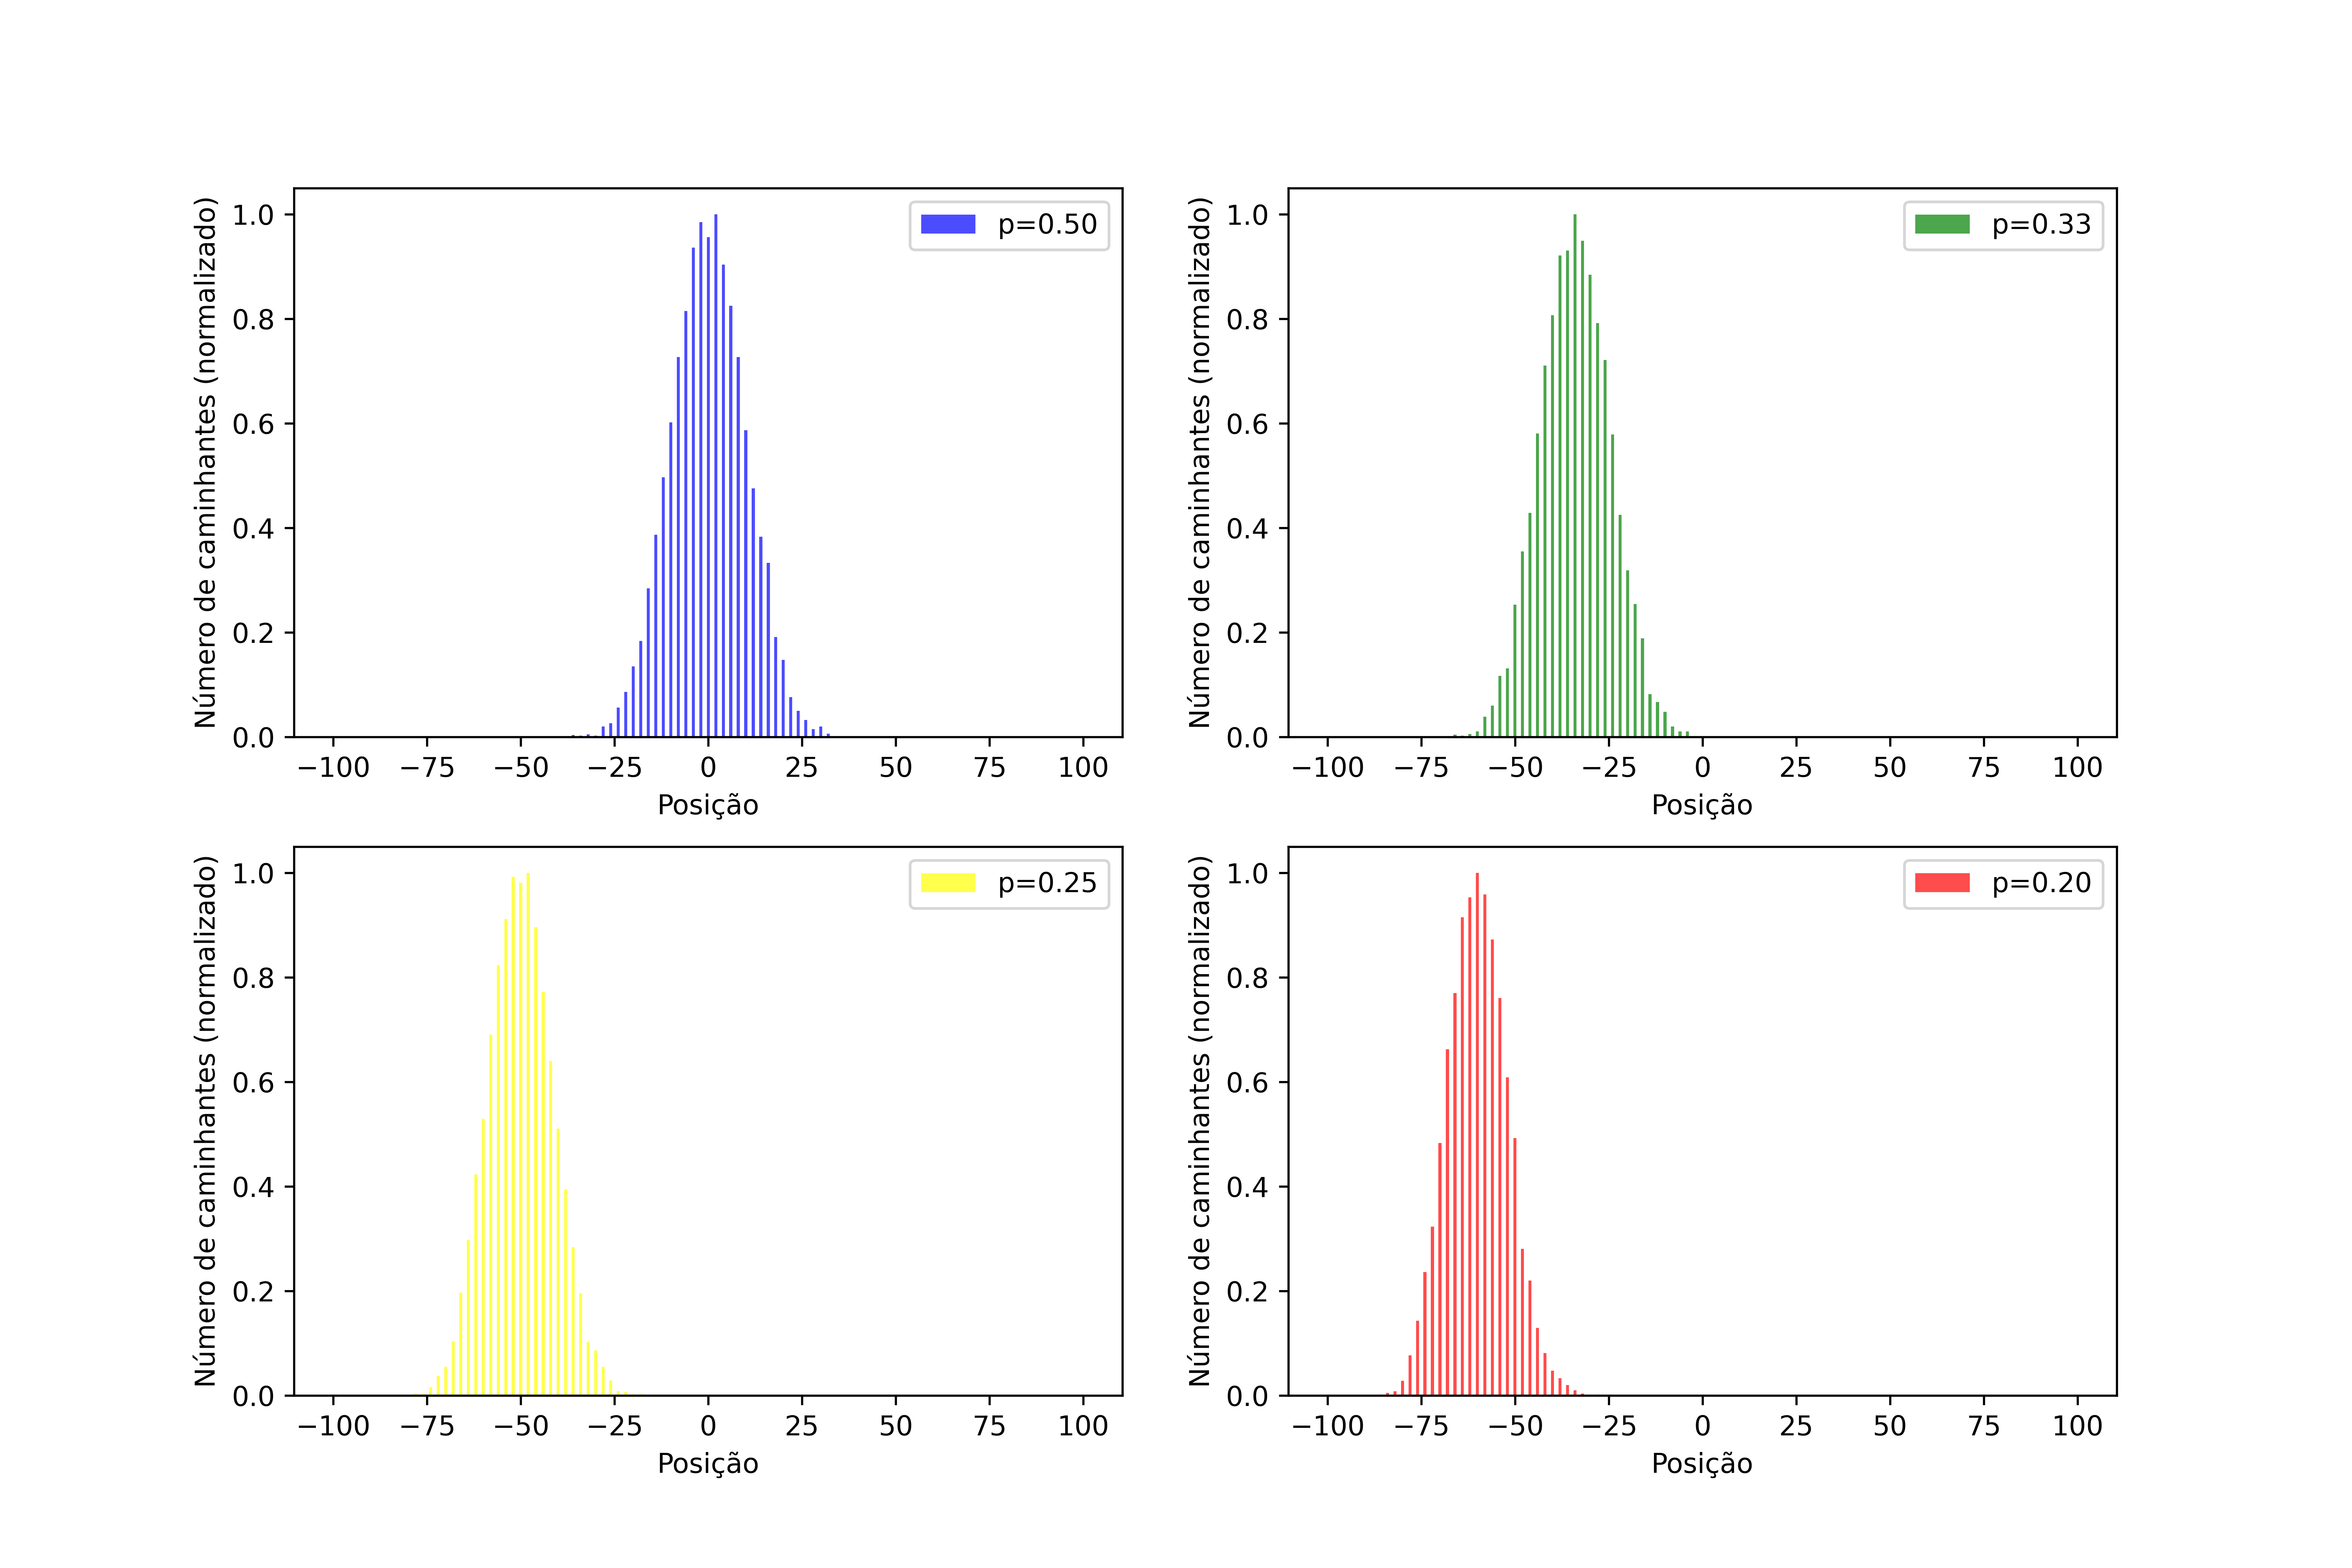
\includegraphics[width=18cm]{images/tarefa-2/plot1.png}
\caption*{Fonte: Compilado pelo Autor.}
\label{fig:histogram1}
\end{figure}



\begin{figure}[h!]
\centering
\caption{Histograma da distribuição de andarilhos em diferentes posições no eixo-x, para $M = 10^4$ e $n=100$.}
  \centering
  % Ensure the image exists at the specified path or update the path below
  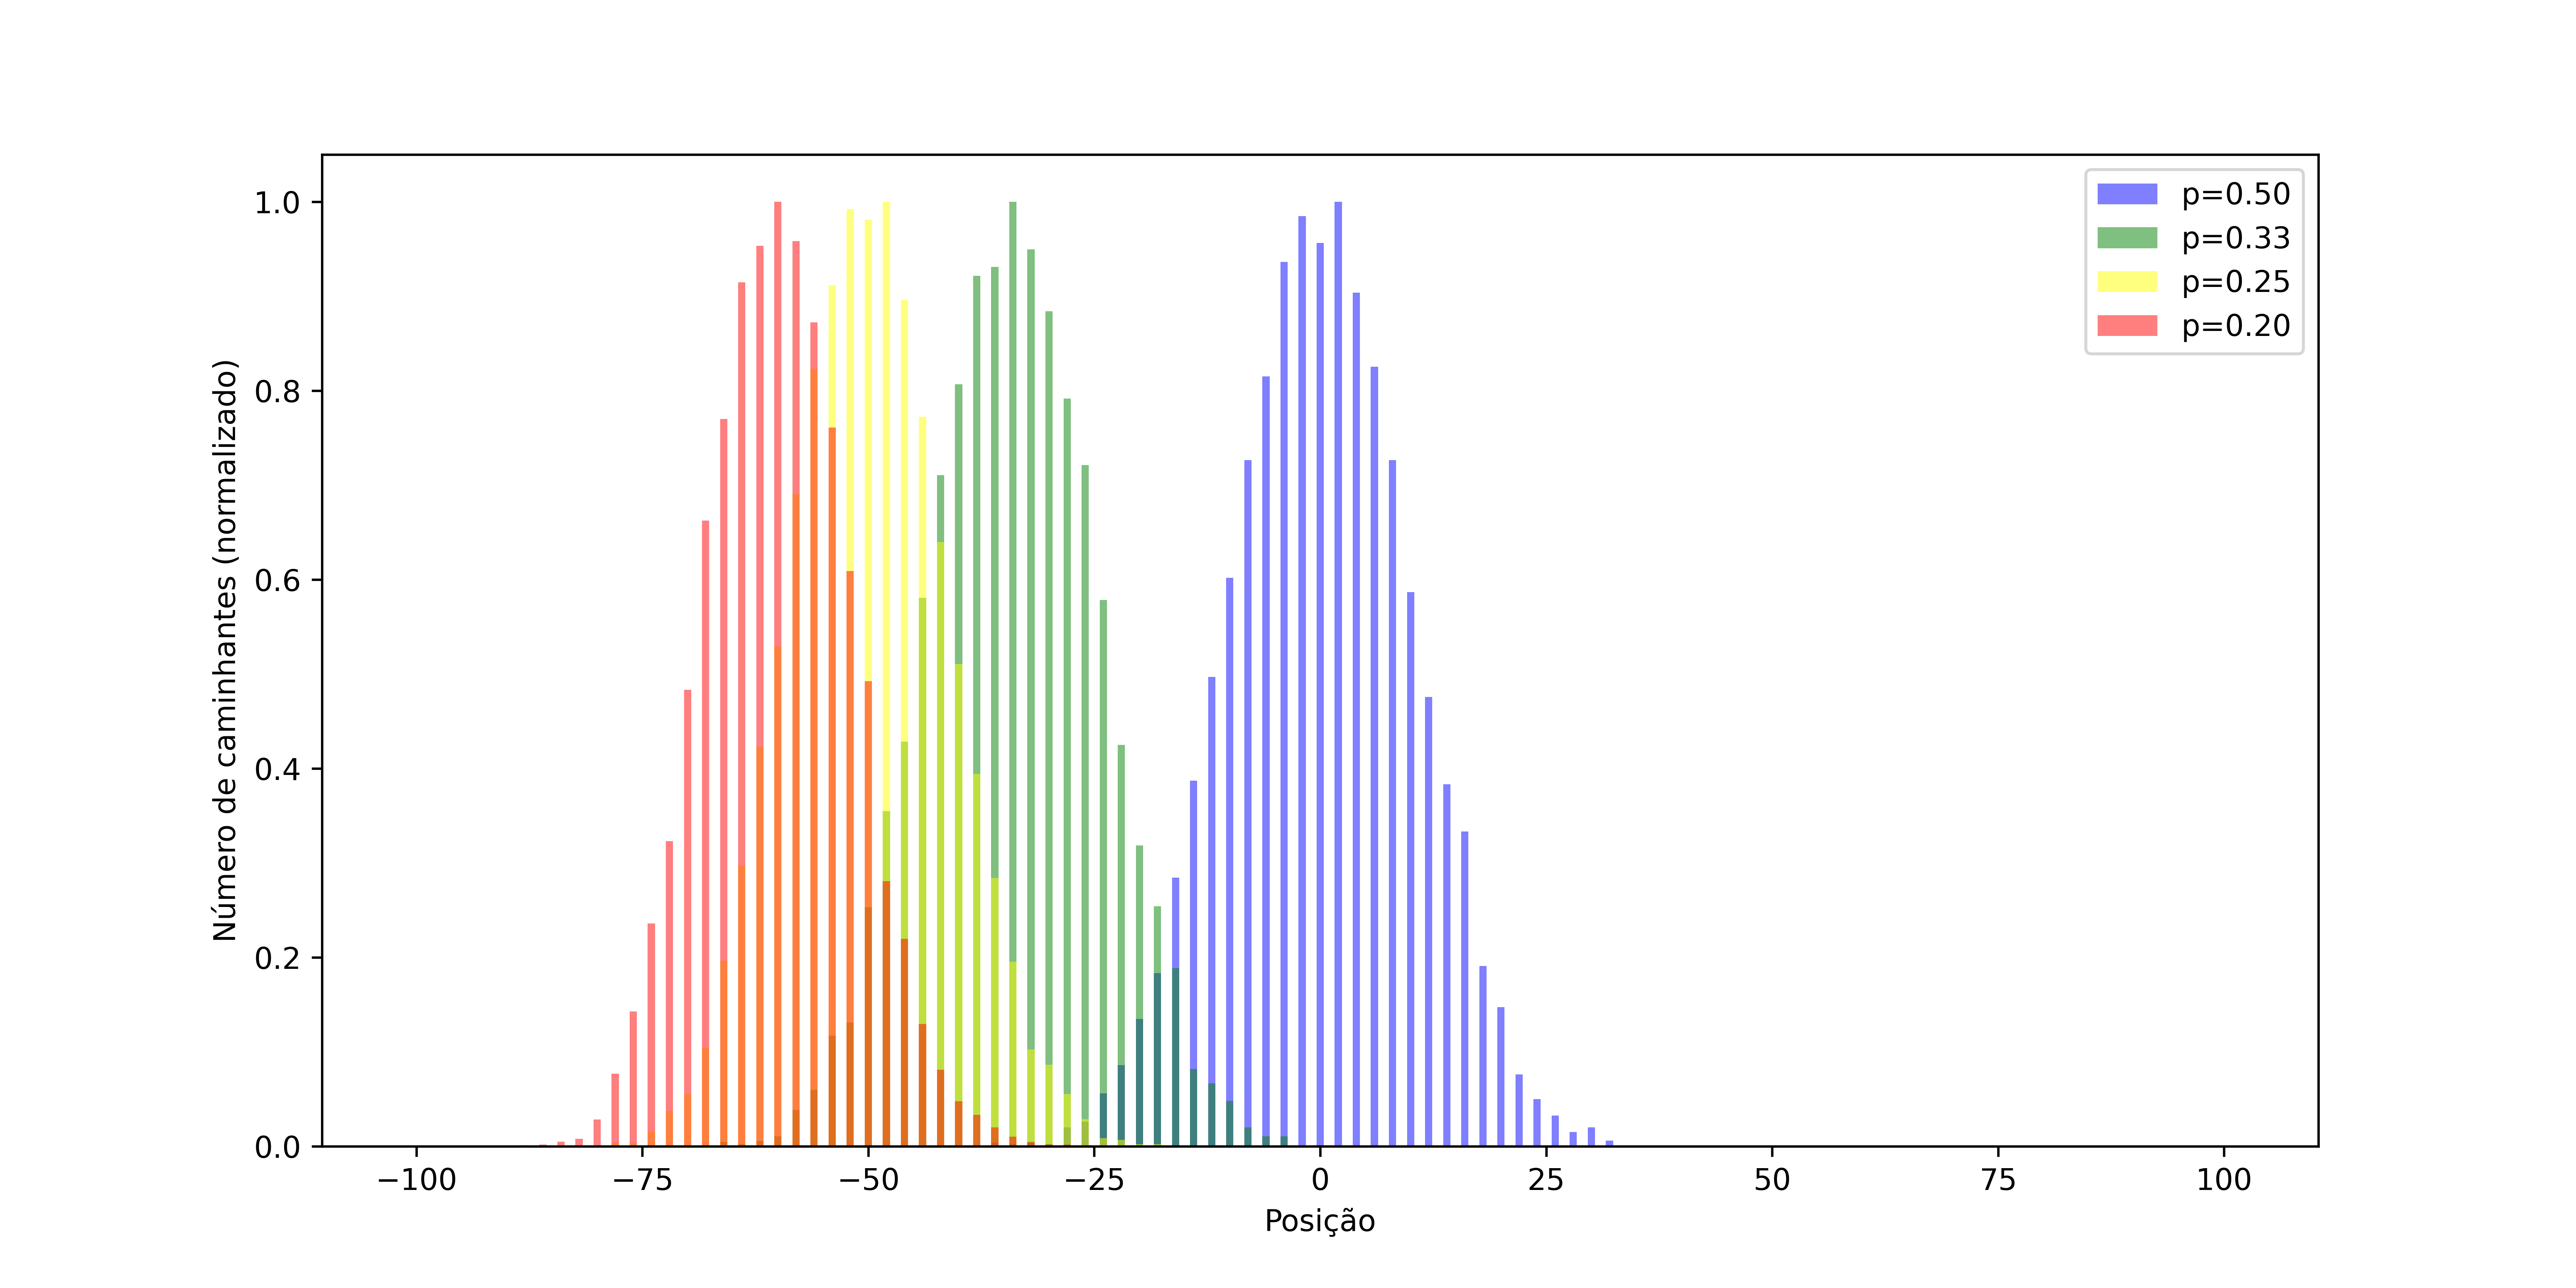
\includegraphics[width=18cm]{images/tarefa-2/plot2.png}
\caption*{Fonte: Compilado pelo Autor.}
\label{fig:histogram2}
\end{figure}

\begin{figure}[h!]
\centering
\caption{Resultado exibido pela simulação no terminal, onde $m=10^4$, $n=100$ e $p=0.50$.}
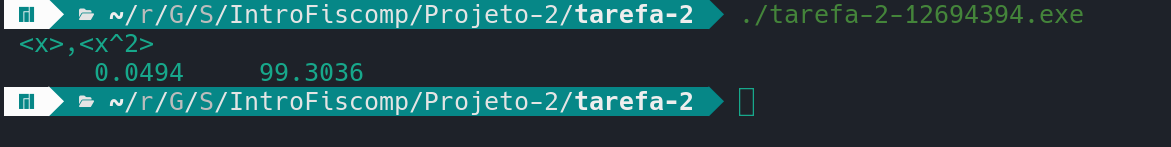
\includegraphics[width=16cm]{images/tarefa-2/terminal-tarefa-2.png}
\caption*{Fonte: Compilado pelo Autor.}
\label{fig:tarefa 2 - terminal}
\end{figure}
